\sectionquestion{Logistic Regression}

\begin{parts}


\part Consider a binary classification problem over labels $y \in \{0,1\}$. In binary logistic regression, we use the sigmoid $\sigma(a)$ function to map real valued scalars to probabilities between 0 and 1. Now suppose we define a new model \emph{binary tanh regression} for the same task by swapping out the sigmoid function for another one: 
\begin{align*}
    p(y=1|\xv,\theta) = \frac{\tanh(\theta^T\xv)+1}{2} 
    \text{ where } 
    \tanh(a) = \frac{\exp(a)-\exp(-a)}{\exp(a)+\exp(-a)}
\end{align*}
A convenient property you may use is that $\tanh(a) = n\sigma(na)-1$ for $n=2$.
\begin{subparts}
    % \subpart[2]{It can be shown that $\tanh(a) = n\sigma(na)-1$ for some integer $n$. What is the value of $n$?} 
    % \begin{tcolorbox}[fit,height=1.5cm, width=4cm, blank, borderline={1pt}{-2pt}]
    %             %solution
    % \end{tcolorbox} 
    % \begin{soln}
    %     Equating both sides we get:
    %     \begin{equation}
    %          \frac{2\exp(x)}{\exp(x)+\exp(-x)} = \frac{2}{1+\exp(-2x)} = \frac{n}{1+\exp(-nx)}
    %     \end{equation}
    %     Thus we get $n=2$
    % \end{soln}
    
    \subpart[2] \textbf{Short answer:} For a single example $(\xv^{(i)},y^{(i)})$, what is the likelihood of this data point under this new model? Your answer should be in terms of $\theta,\sigma,\xv^{(i)},y^{(i)}$, it should not include $n$ or $\tanh$. \textit{For full credit, you must define a single expression without cases. }
    \begin{tcolorbox}[fit,height=2cm, width=15cm, blank, borderline={1pt}{-2pt}]
                %solution
    \end{tcolorbox} 
    \begin{soln}
        \begin{equation}
            L = p(y^{(i)}=1|x^{(i)},\theta)^{y^{(i)}} (1-p(y^{(i)}=1|x^{(i)},\theta))^{1-y^{(i)}}
        \end{equation}
        \begin{equation}
            L = \sigma(2\theta^T x^{(i)})^{y^{(i)}} (1-\sigma(2\theta^T x^{(i)}))^{1-y^{(i)}}
        \end{equation}
    \end{soln}
    
    \subpart[2] \textbf{Short answer:} What is the negative log likelihood for this one example $(\xv^{(i)},y^{(i)})$? Your answer should be in terms of $\theta,\sigma,\xv^{(i)},y^{(i)}$, it should not include $n$ or $\tanh$. 
    \textit{For full credit, you must define a single expression without cases. }
    \begin{tcolorbox}[fit,height=2cm, width=15cm, blank, borderline={1pt}{-2pt}]
                %solution
    \end{tcolorbox} 
    \begin{soln}
        \begin{equation}
            -\log L = -y_i \log(\sigma(2\thetav^T\xv_i)) - (1-y_i)(\log(1-\sigma(2\thetav^T\xv_i)))
        \end{equation}
    \end{soln}

    % SKIPPED FOR TIME:
    %
    % \subpart[3] \textbf{Short answer:} Let $J^{(i)}(\theta)$ denote the negative log likelihood for this one example. What is $\frac{\partial J^{(i)}(\theta)}{\partial \theta_j}$? Your answer should be in terms of $\theta,\sigma,x^{(i)},y^{(i)}$, it should not include $n$ or $\tanh$. \textit{Hint:} Some useful derivatives: $\frac{\partial \sigma(a)}{\partial a} = \sigma(a)(1 - \sigma(a))$ and $\frac{\partial \log(b)}{\partial b} = \frac{1}{b}$.
    % \begin{tcolorbox}[fit,height=4cm, width=15cm, blank, borderline={1pt}{-2pt}]
    %             %solution
    % \end{tcolorbox} 
    % \begin{soln}
    %     \begin{align*}
    %         \frac{\partial J^{(i)}(\theta)}{\partial \theta_j} 
    %         &= \frac{\partial}{\partial \theta_j}\left(  -y_i \log(\sigma(2\thetav^T\xv_i)) - (1-y_i)(\log(1-\sigma(2\thetav^T\xv_i))) \right) \\
    %         &= \frac{\partial}{\partial \theta_j}\left(  -y_i \log(\sigma(2\thetav^T\xv_i)) - (1-y_i)(\log(1-\sigma(2\thetav^T\xv_i))) \right) \\
    %         &= 2(\sigma(2 \thetav^T \xv^{(i)}) - y^{(i)}) x_j^{(i)} 
    %     \end{align*}
    % \end{soln}

    \subpart[2] \textbf{Short answer:} Now consider a dataset of $N$ points $\Dc = \{ (\xv^{(i)},y^{(i)}) \}_{i=1}^N$. Write the update rule for the vector $\thetav$ using gradient descent assuming the objective function to be the average negative log likelihood over the $N$ points. Take the learning rate to be $\eta$. Your answer should be in terms of $\theta,\sigma,\xv^{(i)},y^{(i)}$,$N$,$\eta$, it should not include $n$ or $\tanh$---and it must include the term $\nabla J^{(i)}(\thetav)$ where $J^{(i)}(\theta)$ denotes the negative log likelihood for the $i$th example (i.e. we don't want you to do any calculus here). 
    \begin{tcolorbox}[fit,height=2cm, width=15cm, blank, borderline={1pt}{-2pt}]
                %solution
    \end{tcolorbox} 
    \begin{soln}
        \begin{equation}
            %\theta_j \leftarrow \theta_j - \eta \frac{1}{N} \sum_{i=1}^N 2(\sigma(2 \theta^T x^{(i)}) - y^{(i)}) x_j^{(i)} 
            %\thetav \leftarrow \thetav - \eta \frac{1}{N} \sum_{i=1}^N 2(\sigma(2 \thetav^T \xv^{(i)}) - y^{(i)}) \xv^{(i)} 
            \thetav \leftarrow \thetav - \eta \frac{1}{N} \sum_{i=1}^N \nabla J^{(i)}(\thetav)
        \end{equation}
    \end{soln}
    
\end{subparts}
    \begin{qauthor}
    Pranit, Logistic Regression, Given a discriminative probabilistic model, derive the conditional log-likelihood
    (adapted by Matt)
    \end{qauthor}

 \clearpage
\part Consider the test dataset below for binary classification containing five points, two are labeled $y = +1$ (indicated by a square $\blacksquare$), two are labeled $y = -1$ (indicated by a triangle $\blacktriangle$), and one has unknown label $y \in \{+1, -1\}$ (indicated by a circle $\bullet$, $\xv^{(5)} = (1.0,0.5)$). 
%
We employ a logistic regression model to classify these points according to a modified decision rule: if $\sigma(w^Tx+b) \ge t$ then $y=+1$, otherwise $y=-1$, where the threshold $t \in [0,1]$. Assume that $w=[1,-1]^T$, $b=0$. 
%
Furthermore, you have access to a plot depicting the accuracy of this model across the five points as the threshold $t$ is adjusted. 
%Hint: $\sigma(0.5) = 0.62$, $\sigma(1) = 0.73$, and $\sigma(x)+\sigma(-x)=1$. 
%Answer the questions given below based on this information. 

\begin{minipage}{0.5\linewidth}
    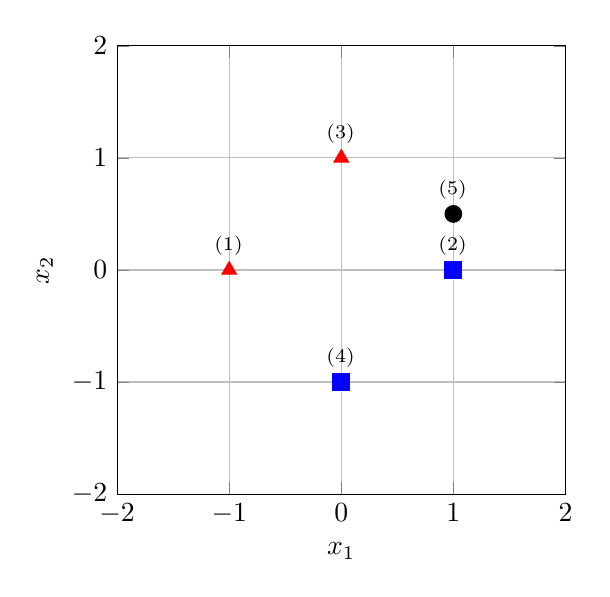
\begin{tikzpicture}
    \begin{axis}[
        scale=1, axis equal image, mark options={scale=1.5},
        xmin=-2, xmax=2, xtick={-2,...,2},
        ymin=-2, ymax=2, ytick={-2,...,2},
        samples=50, grid=major, xlabel=$x_1$, ylabel=$x_2$]]
        \addplot [
            scatter,
            only marks,
            point meta=explicit symbolic,
            scatter/classes={
                a={mark=square*,blue},
                b={mark=triangle*,red},
                c={mark=*,black}
            },
            nodes near coords*={$\xv^{(\pgfmathprintnumber[frac]\myvalue)}$},
            visualization depends on={\thisrow{myvalue} \as \myvalue},
        ] table [meta=label] {
            x y label myvalue
            -1 0 b 1
            1 0 a 2
            0 1 b 3
            0 -1 a 4
            1 0.5 c 5
        };
        %\addplot[ultra thick, color=green] coordinates { (-2,-2) (2,2) };
        %\draw[->, >=stealth, ultra thick, color=green] (axis cs:0,0) -- (axis cs:1,-1);
    \end{axis}
    \end{tikzpicture} 
\end{minipage}
\begin{minipage}{0.5\linewidth}
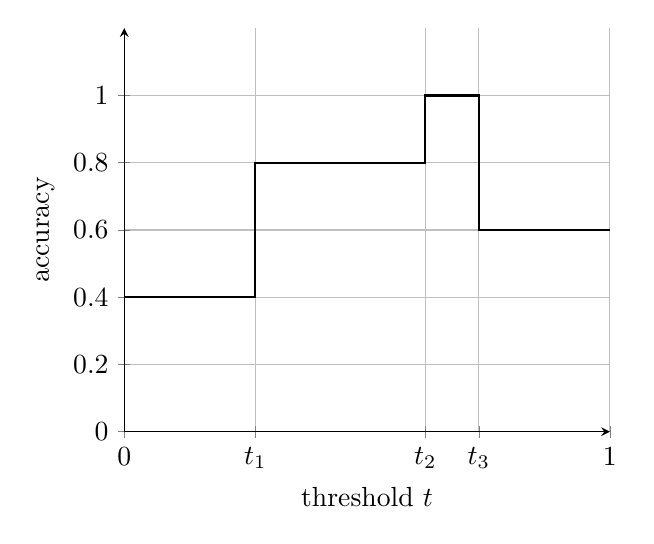
\begin{tikzpicture}
\begin{axis}[
    scale=0.9,
    axis lines = left,
    xlabel = threshold $t$,
    ylabel = {accuracy},
    ymin=0, ymax=1.2,
    xmin=0,xmax=1,
    xtick={0,0.27,0.62,0.73,1},
    xticklabels={0,$t_1$, $t_2$, $t_3$,1},
    ytick={0,0.2,0.4,0.6,0.8,1},
    % xtick={0,1},
    % ytick={0,0.2,0.4,0.6,0.8,1},
    % xticklabels={0,$t_1$,$t_2$,$t_3$},
    % yticklabels={0,0.2,0.4,0.6,0.8,1},
    grid=both,
    ]
    \addplot[const plot, no marks, thick] coordinates {
        (0,0.4) (0.27,0.8) (0.62,1) (0.73,0.6) (1,0.6)
    };

\end{axis}
\end{tikzpicture}
\end{minipage}

\begin{subparts}
    \subpart[1] What is the label of point $x^{(5)}?$ 
    \begin{checkboxes}
        \choice  $y^{(5)} = +1$
        \choice  $y^{(5)} = -1$
    \end{checkboxes}
    \begin{soln}
        Label of $x^{(5)} = -1$\\ 
        From either threshold = 0 or threshold =1, we can see that $x^{(5)}$ will be -1. 
    \end{soln}
    
    \subpart[2] What is the value $a_2$ such that $\sigma(a_2) = t_2$?
    \begin{tcolorbox}[fit,height=1.5cm, width=6cm, blank, borderline={1pt}{-2pt}]
                %solution
    \end{tcolorbox}
    \begin{soln}
        $a_2 = 0.5$ and $t_2 = 0.62$ \\ 
        From either threshold = 0 or threshold =1, we can see that $x^{(5)}$ will be -1. Now, we can see that the accuracy can be 1 only if $x^{(5)}$ is classified correctly.  i.e. when $ \sigma(0.5) \le t \le \sigma(1)$ which gives us the answer.  \\
        Give partial credit for $t \in $
    \end{soln}

    \subpart[2] What is the value $a_3$ such that $\sigma(a_3) = t_3$?
    \begin{tcolorbox}[fit,height=1.5cm, width=6cm, blank, borderline={1pt}{-2pt}]
                %solution
    \end{tcolorbox}
    \begin{soln}
        $a_3 = 1.0$ and $t_3 = 0.73$ \\
    \end{soln}

    \end{subparts}
    \begin{qauthor}
    Pranit, Logistic Regression (LO:  Implement logistic regression for binary or multiclass classification)
    (adapted by Matt)
    \end{qauthor}
    
\begin{comment} 
\part \textbf{Matching:} Consider the three algorithms and four update rules shown below. For any algorithm that requires it, assume we are using a fixed learning rate $\gamma$. Match each algorithm to its update rule. It is possible that multiple algorithms may match to the same rule. Assume the bias term is folded into $\thetav$.
    
    \begin{table}[H]
    \vspace{-.5em}
        \begin{subtable}{.5\linewidth}
            \centering
            \begin{tabular}{p{0.7\linewidth}}
                \toprule
                \textbf{Algorithms:} \\
                \midrule
                (A) SGD for Logistic Regression 
                \newline \hspace*{2em} $\displaystyle h_{\thetav}(\xv) = p(y=1|x)$ \\
                \midrule
                %
                (B) SGD for Linear Regressions
                \newline \hspace*{2em}$\displaystyle h_{\thetav}(\xv) = \thetav^T \xv$ \\
                \midrule
                %
                (C) Perceptron 
                \newline \hspace*{2em} $\displaystyle h_{\thetav}(\xv) = \text{sign}(\thetav^T \xv)$ \\
                 \hspace*{2em} where $\text{sign}(\cdot) \in \{-1, +1\}$ \\
                \bottomrule
              \end{tabular}
        \end{subtable}
        \begin{subtable}{.5\linewidth}
            \centering
            \begin{tabular}{l}
                \toprule
                \textbf{Update Rules:} Each is of the form \\
                $\thetav \leftarrow \thetav - \gv$ where \\
                \midrule
                (1) $\displaystyle g_k = (h_{\thetav}(\xv^{(i)}) - y^{(i)})$\\
                \midrule
                (2) $\displaystyle g_k =  \gamma (h_{\thetav}(\xv^{(i)}) - y^{(i)}) x_k^{(i)}$\\
                \midrule
                %
                %
                (3) $\displaystyle g_k = \frac{1}{1 + \exp \gamma (h_{\thetav}(\xv^{(i)}) - y^{(i)}) }$\\
                \midrule
                %
                (4) $\displaystyle g_k =  \gamma  \frac{1}{N} \sum_{i=1}^N (h_{\thetav}(\xv^{(i)}) - y^{(i)}) x_k^{(i)}$\\
                \bottomrule
            \end{tabular}
      \end{subtable}
      
    \vspace{-.5em}
    \end{table}
    
    {\small 
    \begin{subparts}
        \subpart[1] Which of the following is the correct update rule for Algorithm A?
        \begin{checkboxes}
        \choice Update Rule (1)
        \choice Update Rule (2)
        \choice Update Rule (3)
        \choice Update Rule (4)
        \end{checkboxes}
        \subpart[1] Which of the following is the correct update rule for Algorithm B? 
        \begin{checkboxes}
        \choice Update Rule (1)
        \choice Update Rule (2)
        \choice Update Rule (3)
        \choice Update Rule (4)
        \end{checkboxes}
        \subpart[1] Which of the following is the correct update rule for Algorithm C? 
        \begin{checkboxes}
        \choice Update Rule (1)
        \choice Update Rule (2)
        \choice Update Rule (3)
        \choice Update Rule (4)
        \end{checkboxes}
    \end{subparts}
    }
    \begin{soln}
        \begin{enumerate}
        \item (2)
        \item (2)
        \item (2)
    \end{enumerate}
    \end{soln}
    
    \begin{qauthor}
    Tara (Matt adapted back into a matching question to reduce reading time. Similar to S19 version.)
    \end{qauthor}

\clearpage

\newcommand{\NarName}{Graddyant}
\part \NarName{} the Narwhal\texttrademark\,\textit{really} doesn't like the sigmoid in binary logistic regression and proposes the following binary classification model using softmax instead. Let the input to the model be $\xv \in \mathbb{R}^m$, let the label be $y \in \{ 0, 1 \}$, and let the model weights be $\Av \in \mathbb{R}^{2 \times m}$, where $\Av_1, \Av_2 \in \mathbb{R}^m$ refer to the first and second rows of $\Av$.
\begin{align*}
\zv &= \Av \xv = [\Av_1 \xv, \Av_2 \xv]^T \\
\hv &= \text{softmax}(\zv) = \bigg[ \frac{e^{z_1}}{e^{z_1} + e^{z_2}}, \frac{e^{z_2}}{e^{z_1} + e^{z_2}} \bigg]^T
\end{align*}
Under \NarName{}'s formulation, $h_1$ represents $P(y = 0 \,|\, \xv)$ and $h_2$ represents $P(y = 1 \,|\, \xv)$.
\begin{subparts}
    \subpart \textbf{Fill in the blanks:} Fill in the blanks in the expression below for the log likelihood of a single example $(\xv, y)$. Your answers should be in terms of $\Av_1, \Av_2$ and $\xv$.
    
    \textit{(Hint: Recall for a sample $b$ of a Bernoulli random variable $B$ with parameter $\phi$, we write the likelihood of $b$ as $\phi^b(1-\phi)^{(1-b)}$.)}
    \begin{align*}
        (\blankforFITB{2em}{i.}) \cdot y + (\blankforFITB{2em}{ii.}) \cdot (1 - y) - \log(e^{z_1} + e^{z_2})
    \end{align*}
    \begin{subsubparts}
    \subsubpart[1]
    \begin{tcolorbox}[fit,height=1.5cm, width=6cm, blank, borderline={1pt}{-2pt}, nobeforeafter]
                %solution
    \end{tcolorbox}
    \subsubpart[1]
    \begin{tcolorbox}[fit,height=1.5cm, width=6cm, blank, borderline={1pt}{-2pt}, nobeforeafter]
                %solution
    \end{tcolorbox}
    \end{subsubparts}
    \begin{soln}
    \begin{align*}
        \ell(\Av) &= y \log h_2 + (1-y) \log h_1 \\
        &= y z_2 + (1-y) z_1 - \log(e^{z_1} + e^{z_2}) \\
        &= A_2 x \cdot y + A_1 x \cdot (1-y) - \log(e^{z_1} + e^{z_2})
    \end{align*}
    \end{soln}   
    \begin{qtester}
    We should maybe put a,b on the blank lines and label the corresponding boxes.
    \end{qtester}
    \subpart[1] \textbf{Fill in the blank:} Fill in the decision rule of the Bayes optimal classifier, assuming all mistakes incur a loss of 1. Your answer should be in terms of $z_1$ and $z_2$. If there are ties, you may break them arbitrarily.
    \begin{align*}
        \hat{y} = \begin{cases} 1 & \text{if } \blankforFITB{2em}{} \\ 0 & \text{otherwise} \end{cases}
    \end{align*}
    \begin{tcolorbox}[fit,height=1.5cm, width=6cm, blank, borderline={1pt}{-2pt}, nobeforeafter]
                %solution
    \end{tcolorbox}
    
    \begin{soln}
        $z_2 \geq z_1$ or $z_2 > z_1$ or equivalent
    \end{soln}

\clearpage

    \subpart[3] \textbf{Proof:} Neural claims that \NarName{}'s model yields exactly the same decision boundary as a log regression model $p(y=1 \mid \xv) = \sigma(\thetav^T\xv)$ with weights $\thetav = \Av_2^T - \Av_1^T$. Is Neural right? If yes, show that the decision boundaries are mathematically equivalent. If not, give a specific weight matrix $\Av$ and input $\xv$ that contradicts Neural's statement.
    
    \begin{tcolorbox}[fit,height=7cm, width=15cm, blank, borderline={1pt}{-2pt}]
    %solution
    \end{tcolorbox}

    \begin{soln}
        The decision boundary of log regression is $\sigma(\theta^T x) \geq 0.5 \iff \theta^T x \geq 0 \iff (\Av_2 - \Av_1) x \geq 0 \iff \Av_2 x \geq \Av_1 x \iff z_2 \geq z_1$.
    \end{soln}

    % Matt: Commenting out this subpart as it's not needed here.
    %
    % \subpart[1] \textbf{Numerical answer;} In terms of $m$ (recall that $\xv \in \mathbb{R}^m$), what is the VC dimension of Gradient's model?
    %
    % \begin{tcolorbox}[fit,height=1cm, width=4cm, blank, borderline={1pt}{-2pt}, nobeforeafter]
    % \end{tcolorbox}
    %
    % \begin{soln}
    %     $m$ since we don't have a bias
    % \end{soln}
\end{subparts}
\begin{qauthor}
    Alex \\
    Given a discriminative probabilistic model, derive the conditional log-likelihood, its
gradient, and the corresponding Bayes Classifier \\
    Technically we don't have a learning objective for VC dimension - is it still fair game?
\end{qauthor}

\begin{qtester}
I think VC dimension would be fair game, but we should check with Matt. I also wonder if this question is a bit long with the amount of reading along with a derivation. 
\end{qtester}
\begin{qauthor}
    I don't mind deleting some parts of the question, the main reason I wrote it was for the decision boundary question in part (c).
\end{qauthor}


\part Suppose we are performing logistic regression, with $p(y=1|\xv,\thetav) = \sigma(\thetav^T \xv)$ (no intercept term). Normally, the decision rule for classifying a data point as a positive is $\sigma(\thetav^T \xv) \ge 0.5$, and we say that the \textit{threshold of classification} is 0.5 in this case. 
Suppose we instead use a \emph{modified} decision rule that classifies as positive when $p(y=1|\xv,\thetav) \ge t p(y=0|\xv,\thetav)$ where $t$ is a scalar such that $ t > 0 $. 
\begin{subparts}
    \subpart[2] \textbf{Derivation:} What is the \emph{modified} threshold of classification in terms of $t$? Show your work in the box below and circle your final answer for the threshold.
   
    
    \begin{tcolorbox}[fit,height=7cm, width=15cm, blank, borderline={1pt}{-2pt}, nobeforeafter]
    \end{tcolorbox}

    \begin{soln}
    \begin{equation}
         p(y=1|x,\theta) \ge tp(y=0|x,\theta)
    \end{equation}
    \begin{equation}
        p(y=1|x,\theta) \ge t(1-p(y=1|x,\theta))
    \end{equation}
    \begin{equation}
        p(y=1|x,\theta) \ge \frac{t}{t+1} \implies \sigma(\theta^Tx) \ge \frac{t}{t+1}
    \end{equation}

    \end{soln}
    \begin{qauthor}
    Pranit
    \end{qauthor}
    \begin{qtester}
    I like this, but it seems a bit difficult for the 601 exam. we would also need to allow more space for student work. 
    \end{qtester}

    % Matt: removed b/c this part is out of scope.
    % 
    % \subpart[1] \textbf{Fill in the blank:} Let the modified decision boundary be $\theta^Tx + f(t) = 0$, where $f(t)$ is a function of $t$. What is $f(t)$? Is $f(t)$ convex?

    % \begin{tcolorbox}[fit,height=1cm, width=4cm, blank, borderline={1pt}{-2pt}, nobeforeafter]
    % \end{tcolorbox}

    % \begin{soln}
    % \begin{equation}
    %     \sigma(\theta^Tx) = \frac{t}{t+1}
    % \end{equation}
    % \begin{equation}
    %     \frac{1}{1+\exp(-\theta^Tx)} = \frac{t}{t+1}
    % \end{equation}
    % \begin{equation}
    %     t + 1 = t + t\exp(-\theta^Tx)
    % \end{equation}
    % \begin{equation}
    %     \theta^Tx - \log(t) = 0 \implies f(t) = -\log(t)
    % \end{equation}
    % Yes $f(t)$ is convex. 
    % \end{soln}

    % \begin{qauthor}
    % Pranit
    % \end{qauthor}
    % \begin{qtester}
    % This seems a bit difficult for the 601 exam. we would also need to allow more space for student work. 
    % \end{qtester}

\clearpage

\subpart[2] \textbf{Select all that apply:} Which of the following are true of the modified decision rule?
    {%
    \checkboxchar{$\Box$} \checkedchar{$\blacksquare$} % change checkbox style locally
    \begin{checkboxes}
     \choice For lower values of t (close to 0) there will be very few false negative predictions by the modified decision rule. (A false negative is when we mistakenly predict negative.)
     \choice For very large values of t ($>> 1$) there will be a large number of false positive predictions by the modified decision rule. (A false positive is when we mistakenly predict positive.)
     \choice Using $t=\frac{1}{2}$ returns the standard logistic regression model. 
     \choice The modified decision boundary will only be linear if $t > \frac{1}{2}$.
     \choice None of the above
    \end{checkboxes}
    }
    \begin{soln}
    A \\ 
    A is true because lower values of $t$ will make the model classify almost all points as positives, and hence the recall will be very high with low false negatives. \\
    B is false because large values of $t$ means that very few points will be classified as positives, and thus the precision will be very high. \\ 
    C is false because $t=1$ returns the usual logistic regression model \\ 
    D is false because the decision boundary is always linear
    \end{soln}

    \begin{qauthor}
    Pranit, Prove that the decision boundary of binary logistic regression is linear, 
    \end{qauthor}

\end{subparts}
\end{comment}

\end{parts}